
\section{Propiedades de pérdida}

Es necesario conocer para qué coeficiente de sustentación $C_L$ y ángulo de ataque el ala entra en pérdida $\left( C_{L\text{s}}, \ \alpha_\text{s} \right)$. 

Cada sección del ala tiene un coeficiente de sustentación máximo $\left( C_{l\,\text{max}} \right)$, a partir del cual se da la entrada en pérdida. Según \cite{aerotools_1}, para $\reynolds = 6 \cdot 10^5$ y $10^6$, los $C_{l\,\text{max}}$ son $1.1481$ y $1.0932$, respectivamente. Estos se corresponden con las secciones de raíz y de punta de ala. Dado el estrechamiento lineal, los $C_{l\,\text{max}}$ de cada sección a lo largo de la envergadura se obtienen interpolando linealmente.

El $C_{L\text{s}}$ se puede obtener con las distribuciones de sustentación básica y adicional. Imponiendo $C_l(y) = C_{l\,\text{max}}(y)$ en \eqref{eq:cl_seccion_distribuciones}, el $C_L$ para el que cada sección entra en pérdida es
\begin{equation}
    C_{L\text{s}}(y) = \frac{C_{l\,\text{max}}(y) - C_{l_b}(y)}{C_{l_a}(y)}
\end{equation}
El mínimo de los $C_{L\text{s}}(y)$ $\left( C_{L\text{s} \, \text{min}} \right)$ es $C_{L\text{s}}$, pues para $C_L > C_{L\text{s} \, \text{min}}$ más secciones del ala entran en pérdida.

Calculando la regresión de $C_L = f (\alpha)$, se puede obtener $\alpha_\text{s}$. Suponiendo vuelo horizontal rectilíneo uniforme, \ie, $L = W$, la velocidad de entrada en pérdida es
\begin{equation}
    V_\text{s} = \sqrt{\frac{2 W}{\rho S C_{L\text{s}}}} = 
    \sqrt{\frac{2 g_0 \cdot \mathcal{W}/S}{\rho C_{L\text{s}}}}
\end{equation}

En la figura \ref{fig:stall_lift_distribution} se representa el coeficiente de sustentación local en la entrada en pérdida, el coeficiente de sustentación del ala necesario para la entrada en pérdida de cada sección y las primeras secciones en entrar en pérdida.

\begin{figure}[h]
    \centering
    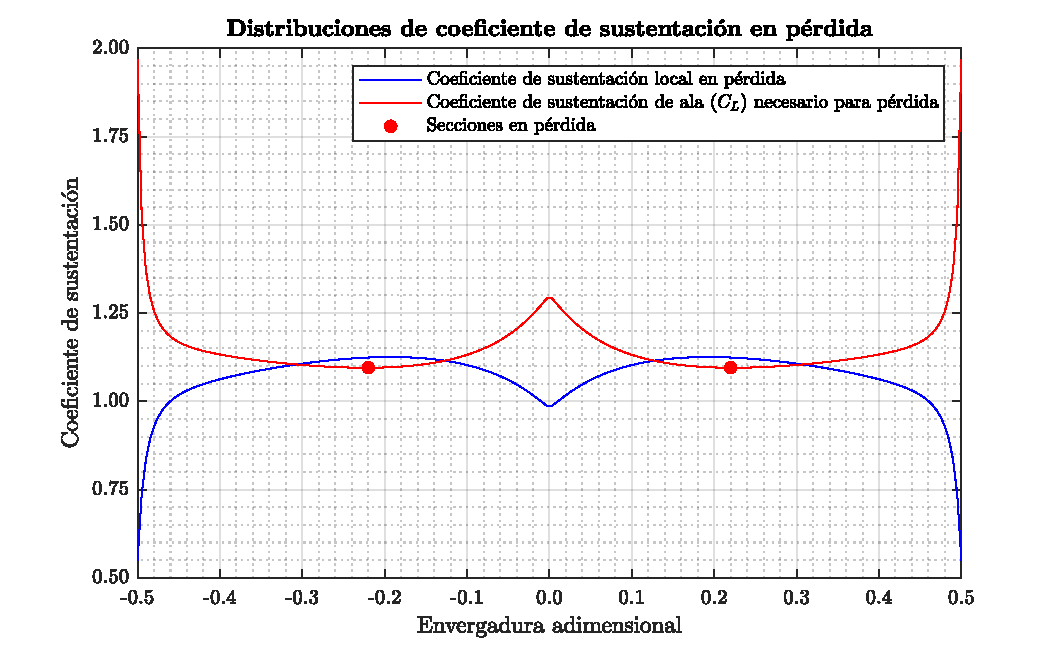
\includegraphics[width=\linewidth]{imagenes/propiedades_perdida/stall_lift_distribution.pdf}
    \caption{Coeficiente de sustentación local $\left( C_l(y) \right)$, coeficiente de sustentación del ala necesario para la entrada en pérdida de la sección $\left( C_L(y_s) \right)$ y primeras secciones en pérdida.}
    \label{fig:stall_lift_distribution}
    \vspace{-4mm}
\end{figure}

Numéricamente, se obtiene que el ala entra en pérdida cuando $C_L = 1.0951$, con un ángulo de ataque $\alpha_\text{s} = 12.85 \degrees$. En VHRU la pérdida se da a $V_\text{s} = 61.6 \ \kilo\meter / \hour$.